\documentclass[12pt]{paper}
\usepackage{amsmath}
\usepackage{amssymb}
\usepackage{graphicx}
\usepackage{hyperref}
\usepackage{color}
\usepackage{float}
\begin{document}
     
\title{Simulating the formation of TADs - Report}
\maketitle
In this document we explore through simulations the conditions required for the appearance of the Topologically Associating Domains (TADs). The observation of such regions is reported in Nora et al 2012 as the results of the HiC experiments of the genomic region including the X inactivation center of the X chromosome. Experimental data is supplied by L. Giorgetti as a subset of the experimental data obtained in Nora et. al 2012. To have a good ground for comparison, we follow data coarse-graining procedure as described in the supplementary material of Giorgetti et al 2014, which transforms the segment encounter data to those of beads by dividing the genome into equal parts of 3000 bp.   

\section{The Simulation Framework}
We have constructed a stochastic simulation framework, which allows the examination of the behavior of the polymer chain in various configurations.
We use the Rouse model to mathematically describe the polymer chain as a series of beads connected by harmonic springs. The stochastic differential equation describing the dynamics of bead $n$ in a chain of $N$ beads is 
\begin{equation*}
\frac{dR_n}{dt} = -D\nabla_{R_n}\phi_{Rouse}+\sqrt{2D}\frac{dw_n}{dt}
\end{equation*}
with the potential 
\begin{equation*}
\phi_{Rouse}=\frac{\kappa}{2}\sum_{n=1}^N \left(R_n-R_{n-1}\right)^2
\end{equation*}
 which in the linear chain case gives rise to the set of equations

\begin{equation*}
\frac{dR_n}{dt}= -\frac{d\kappa D}{b^2}\left(2R_n-R_{n+1}-R_{n-1}\right)+\sqrt{2D}\frac{dw_n}{dt}
\end{equation*}
for the inner beads, and 
\begin{eqnarray*}
\frac{dR_1}{dt}&=& -\frac{d\kappa D}{b^2}\left(R_1-R_{2}\right)+\sqrt{2D}\frac{dw_1}{dt}\\
\frac{dR_N}{dt}&=& -\frac{d\kappa D}{b^2}\left(R_N-R_{N-1}\right)+\sqrt{2D}\frac{dw_N}{dt}
\end{eqnarray*} 
for the end beads. Where $R_n$ are the coordinates of the $n^{th}$ bead, $d$ is the dimension, $\kappa$ is the spring constant, $D$ is the diffusion constant, $b$ is the standard-deviation of the distance between adjacent beads, and $w$ is N-dimensional white Gaussian noise with mean 0 and variance 1 in each component. 

The flexibility of our framework enables us to simulate a single or an ensemble of chains in open space or in 3 types of domains: a sphere, a cylinder, and between two infinite plates. As an extension to the classical Rouse model, we can also simulate the chain with variable minimal distance, $l_0>0$, between adjacent beads. Hence, we modify the Rouse potential to read
\begin{equation*}
\phi_{Rouse}=-\frac{\kappa}{2}\sum_{n=1}^N\left((\|R_n-R_{n-1}\|-l_0)^2\right)
\end{equation*}
and simulate the coupled (coordinate-wise) system of equations it yields.

In addition, non-adjacent beads can be fixed to form stable loops throughout the simulation. We extend this idea to allow the formation and dissociation of loops in time, a model termed dynamic loop model.
At the end of simulations, an analysis is performed to calculate the encounter probability between beads of the chain, and a report is generated.  

We consider that two beads $R_i$ and $R_j$ had encountered if
\begin{equation*}
 dist_{ij}=\|R_i-R_j\|\leq \epsilon
\end{equation*}
with $0<\epsilon <b$. The theoretical encounter probability in a linear Rouse chain is given by 
\begin{equation}
Pr(dist_{ij}<\epsilon)= \alpha |i-j|^{-1.5}
\end{equation}
with $\alpha>0$. 

At the end of simulations we extract the encounter histogram of beads and fit it with a function of the form 
\begin{equation*}
Pr(dist_{ij}\leq \epsilon)=\alpha_{ij}|i-j|^{-\beta}
\end{equation*}
for each pair of beads in the chain. 

\section{Analysis of the Experimental data}
In our analysis we use the coarse-grained interpretation of the data as performed by Giorgetti et al 2014.  A genomic strand of of 92,432 bp, was equally divided into 3000bp beads, according tot he mean size of the restriction fragments of HindIII enzyme (see Giorgetti et al supplementary material). This coarse-graining resulted in a polymer chain of 307 beads of length 3000 base-pairs each. This genomic region corresponds to the areas of the TADs D (108 beads) and E (199 beads) as presented in Nora et al 2012. 

The basis for the analysis of the experimental data is the encounter matrix. This is a 307 by 307 matrix containing the pair-wise encounter frequencies between beads of the chain in roughly 8 million cells. Calculation of the bead encounter probability then follows these simple steps
\begin{enumerate}
\item for row $i$ (corresponds to bead $i$), average encounter frequencies at an equal distance from bead $i$. i.e. sum cell $i-m$ and $i+m$, to produce the single sided encounter frequency.
\item divide the results by the total sum of encounters for bead $i$, yielding bead encounter probabilities as a function of distance in bead units. 
\item fit a function of the form $\alpha d^{-\beta}$, with $\alpha = \frac{1}{\sum_{j=1}^k j^{-\beta}}$, and $d$ is the distance in bead units, and $\beta$ the parameter to be determined.
\end{enumerate}
     
\section{Simulations}
In this section we present the results of simulation we have performed for various configuration of the chain. 
Simulations are performed for a chain of 64 beads unless stated otherwise. Although the experimental data consist of longer chain, we simulate 64 bead chains as it is a good trade-off between running time and acquiring a good statistical sample group. Due to the properties of Gaussian chain such as the Rouse mode, the concepts shown in our simulation results should not differ much when length of the chain increases.

All simulation were made until relaxation time of the slowest Rouse mode

\subsection{One, two and Three loops at fixed positions}
Here we present \textit{in-silico} experimental results conducted for the case of fixed 1,2, and 3 loops, i.e. beads connected to form loops remain the same throughout the simulations. We use a polymer composed of 64 beads and sequentially simulate the model with loops between bead [10 19], [28 37] and  [46 55] of the linear chain. For each number of loops, 10,000 simulations were performed.

The encounter histograms are presented in Figure \ref{encounterHistogram123Loops} The mean encounter probability calculated for each case is shown in Figure \ref{encounterHistogram123Loops}. The encounter data was fitted with a function of the form $\alpha x^{-\beta}$. The beta values are reported in the legend of Figure \ref{encounterHistogram123Loops}. Since the loops length was set to 9, the encounter probability for the three cases, as a function of distance, shows an increase around distance 9. The values of the probability at that distance are 0.03, 0.034, and 0.035, for 1, 2 and 3 fixed loops respectively. 
\begin{figure}[H]
\centering
\hspace{-72pt}
\vspace{-40pt}
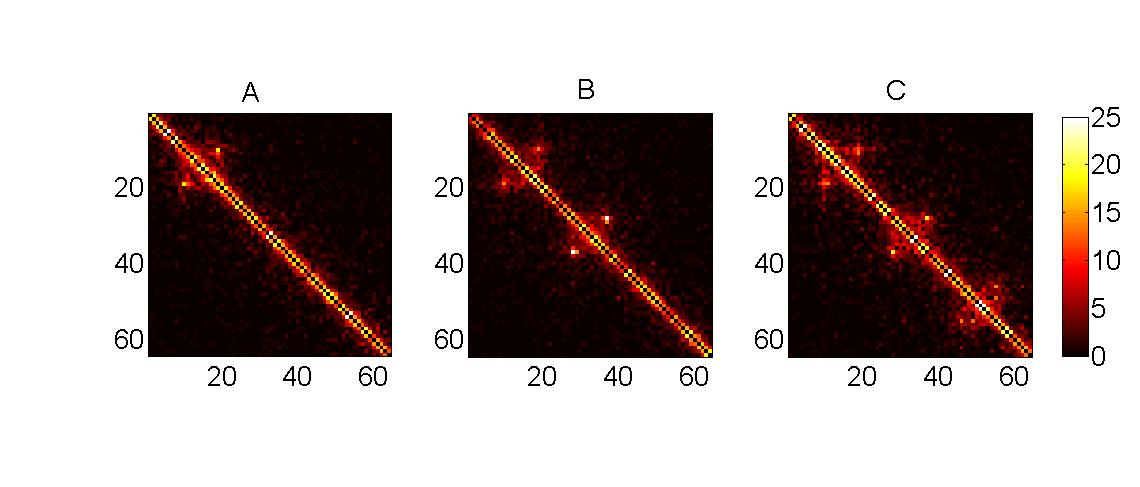
\includegraphics[scale=0.4]{encounterHistogram123Loops}
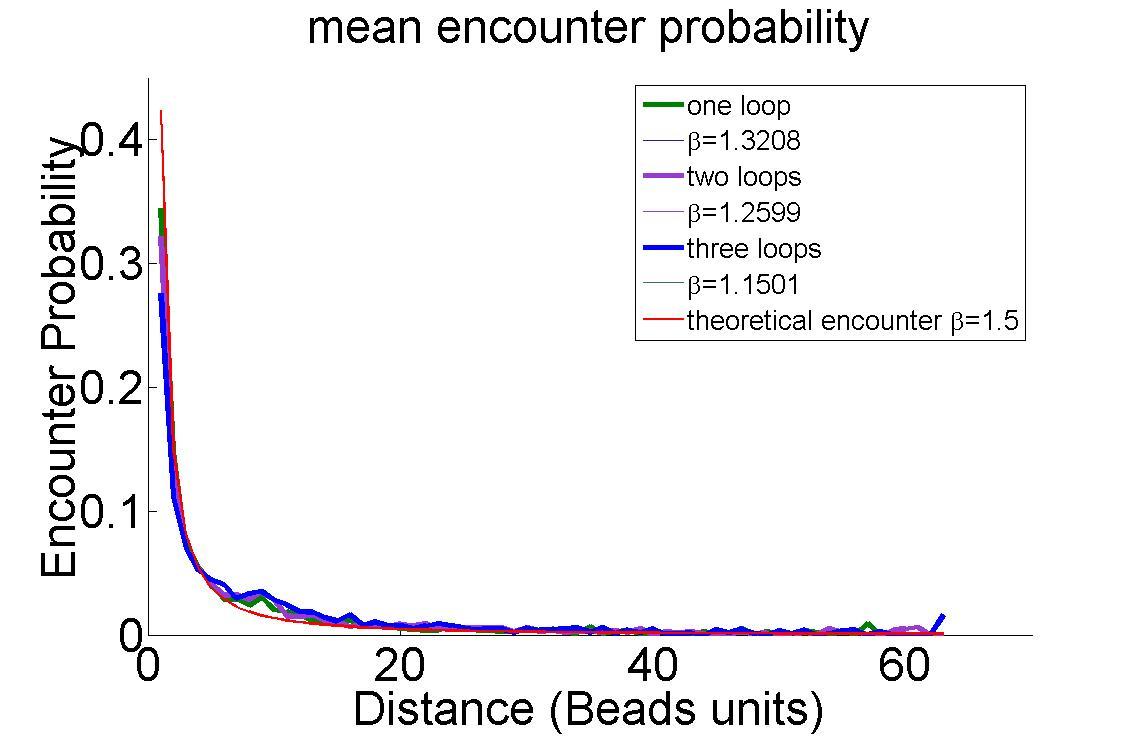
\includegraphics[scale=0.2]{meanEncounterProbability123Loops}
\caption{\scriptsize{The encounter histograms (upper panel) of the 3 fixed position loops cases. (A) a single loop between beads [10 19]. (B) two loops in [10 19], [28 37]. (C) three loops in [10 19],[28 37], and [46 55]]. Each point in the 64 by 64 matrices above represent number of encounters between bead $i$ and $j$. The mean encounter probability (lower panel) for the 3 fixed loops cases: one fixed loop (green), 2 fixed loops (purple), and 3 fixed loops (blue). The fitted $\beta$ values  for the 3 cases are reported in the legend. The theoretical encounter probability curve ($\beta=1.5$) is shown in red. The bump around distance 9 indicates shows the higher encounter probability for the three cases, since the length of each loop was set to 9.}}
\label{encounterHistogram123Loops}
\end{figure}


\subsection{Internal loops}
We now turn to examine the encounter probability of a model containing one 'big' loop when internal loops are sequentially added in it (see Figure \ref{encounterHistogram1To10InternalLoops} lower right panel).  
That is, we connect bead $i$ and $j$ ($j>>i$) and add $n$ loops at of random lengths between bead $i+1$ and bead $j-1$, with the constraint that any bead cannot be connected to form more than one loop. 

For the results presented here, we chose the beads 5 and 60 to form the big loop, we perform 10 simulation rounds, in each we increase the number of internal loops from 1 to 10. The connected beads forming the internal loops are chosen at random. Encounter histogram for the 10 cases are shown in Figure \ref{encounterHistogram1To10InternalLoops} (upper panel). As the number of internal loops is increased, the encounter probability between beads in the loop increases.

The calculated mean encounter probabilities  for the 10 cases are presented in Figure \ref{encounterHistogram1To10InternalLoops} (lower left panel)
\begin{figure}[H]
\centering
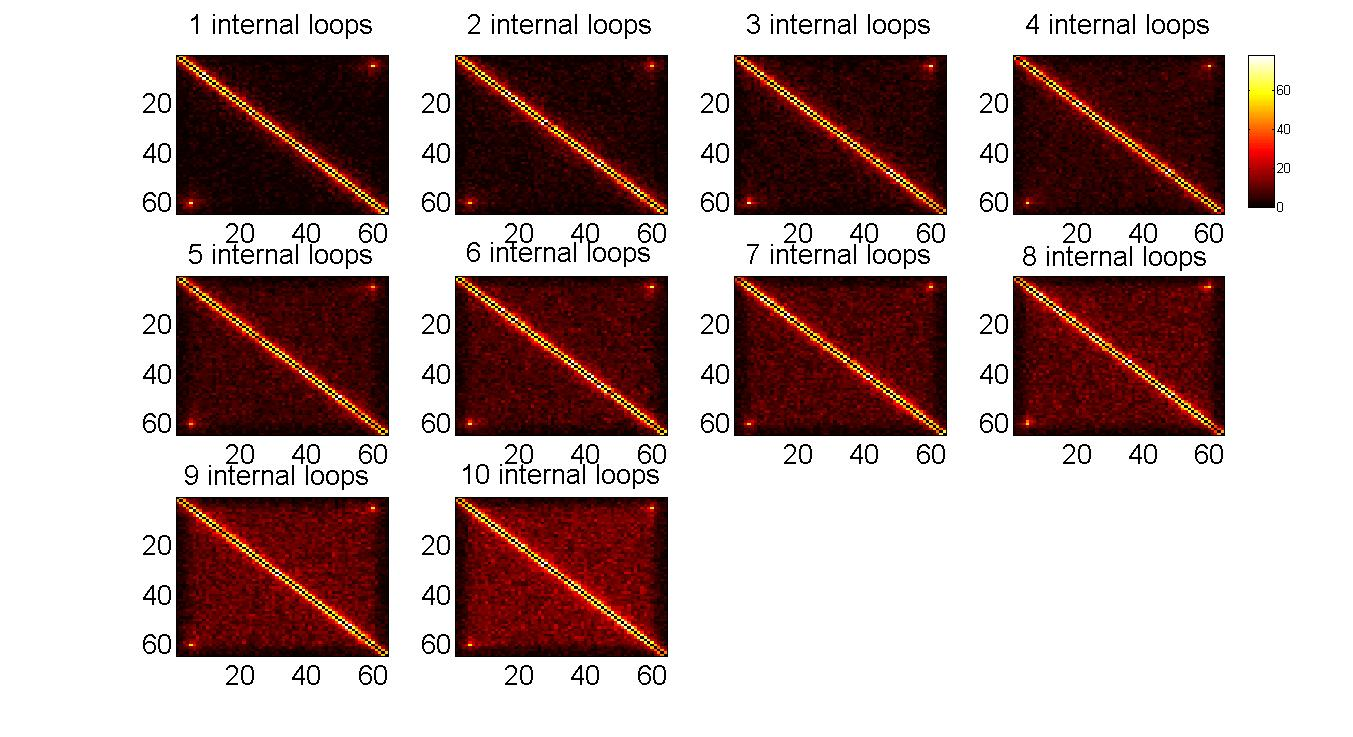
\includegraphics[scale=0.3]{encounterHistogram1To10InternalLoops}
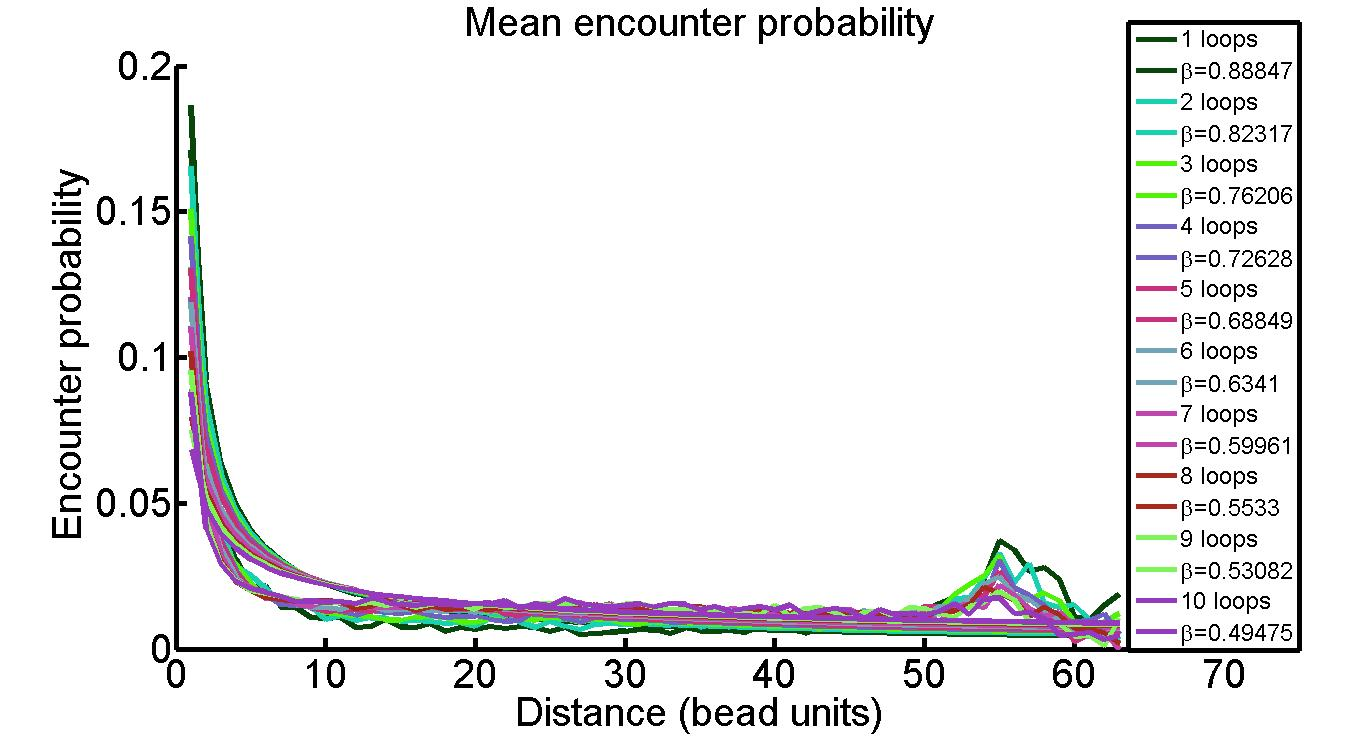
\includegraphics[scale=0.15]{meanEncounterProbabilityInternalLoops}
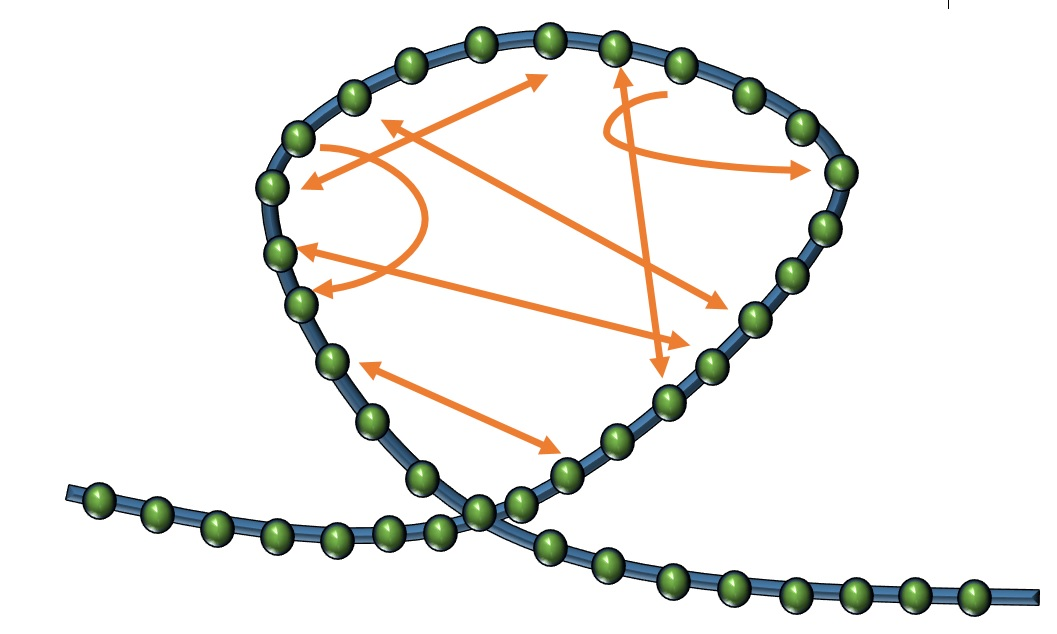
\includegraphics[scale=0.2]{polymerModelWithLoopAndInternalConnectors}
\caption{\scriptsize{The encounter histogram (upper panel) of the model with one big loop between beads 5 and 60, when 1 to 10 internal loops are added to it. The mean encounter probabilities curves (lower left panel) as the number of internal loops is increased from 1 to 10. The simulated encounter data was fitted with a function of the form $\alpha x^{-\beta}$,where $x=1..63$ is the distance in beads units. The bump in distance 55 represents the connection between bead 5 and 59, which constitute the 'big' loop in our simulations and is seen as a consistent bright spot in the encounter histogram (upper panel). A cartoon of the looped model (lower right panel) with internal loops ,arrows indicate the beads to be connected}}
\label{encounterHistogram1To10InternalLoops}
\end{figure}


\subsection{Random fixed loops}
In this experiment we add random length loops between bead $i$ and $j$. We term the range of beads between $i$ and $j$ as a TAD. 

\subsubsection{One TAD}
To simulate a TAD, we employ the random fixed loop model and restrict the bead pairs forming the loops to take indices between beads 1 to 32, the second half of the chain remains a linear Rouse chain. No bead can participate in forming more than one loop. 
We sequentially add 1 to 8 random fixed loops in the region of the TAD, matching the case of two to 16 beads participating in loop formation. 

\begin{figure}[H]
\centering
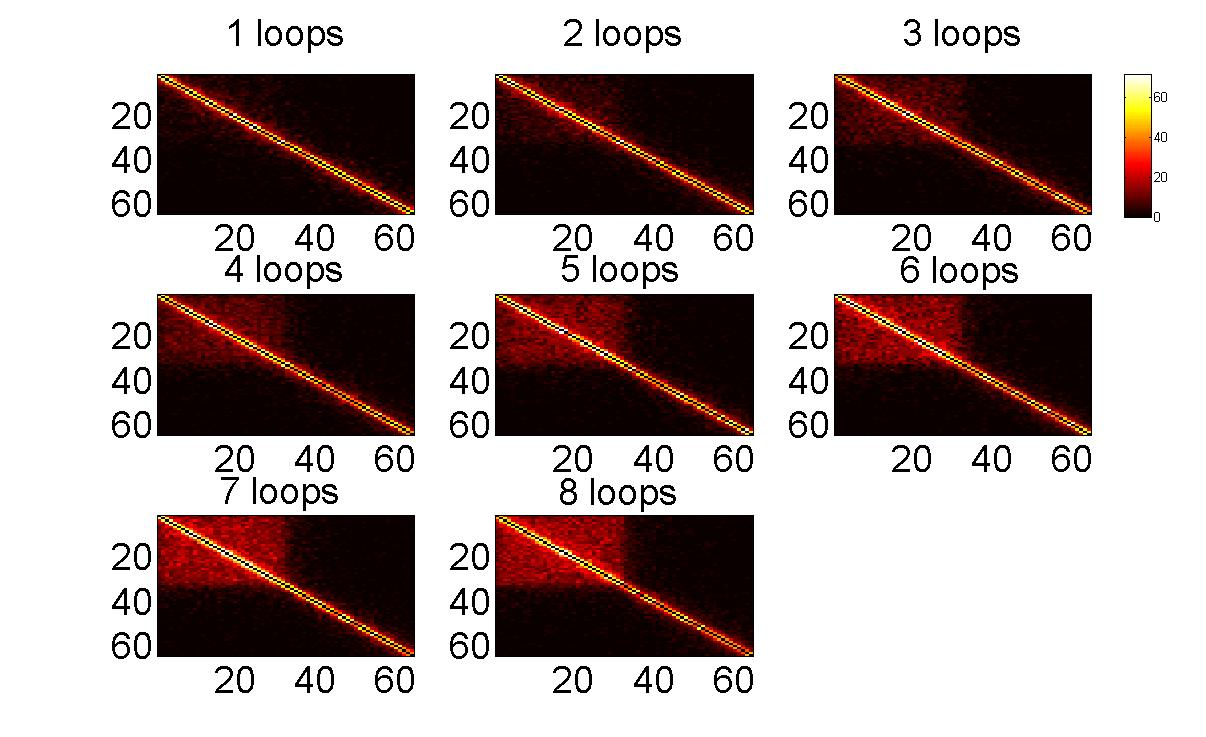
\includegraphics[scale=0.25]{encounterHistogram_1to8Loops}
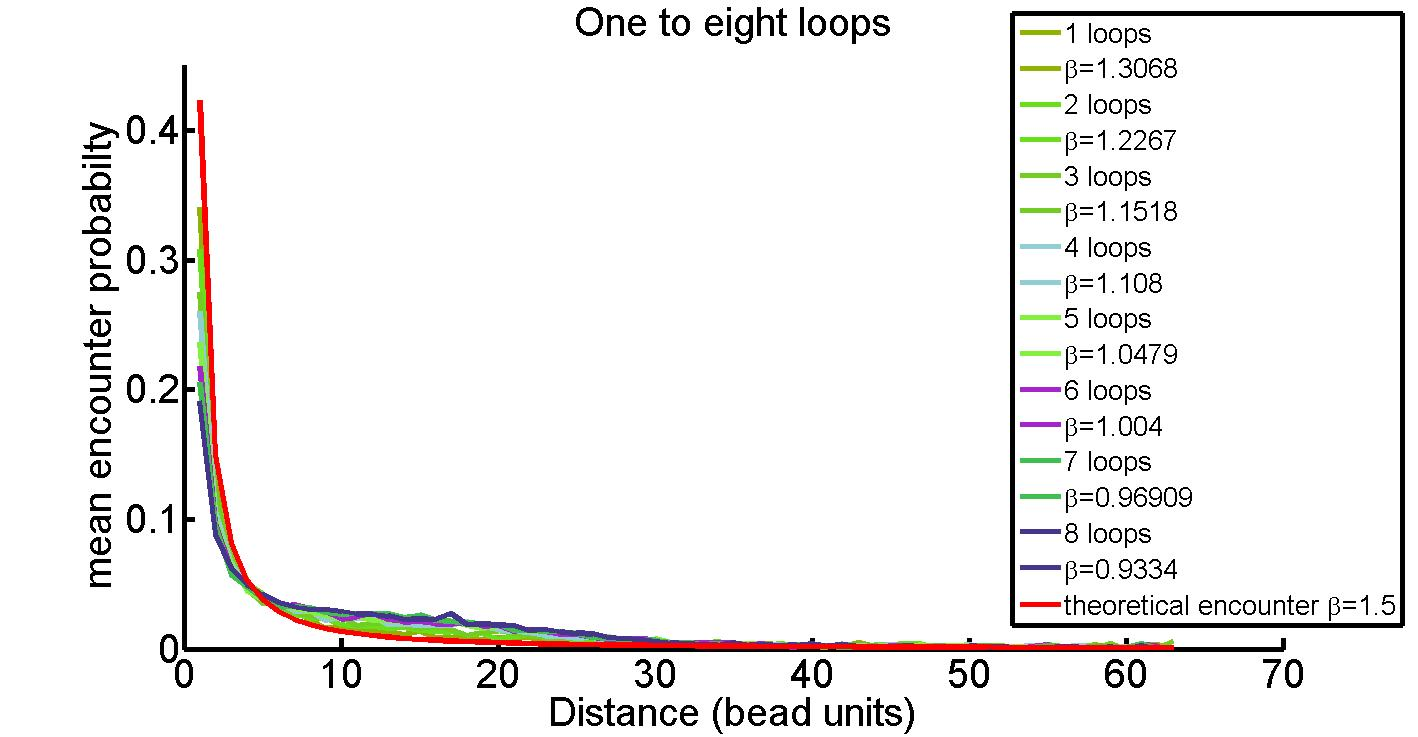
\includegraphics[scale=0.12]{meanEncounterProbabilityOneTAD1To8Loops}
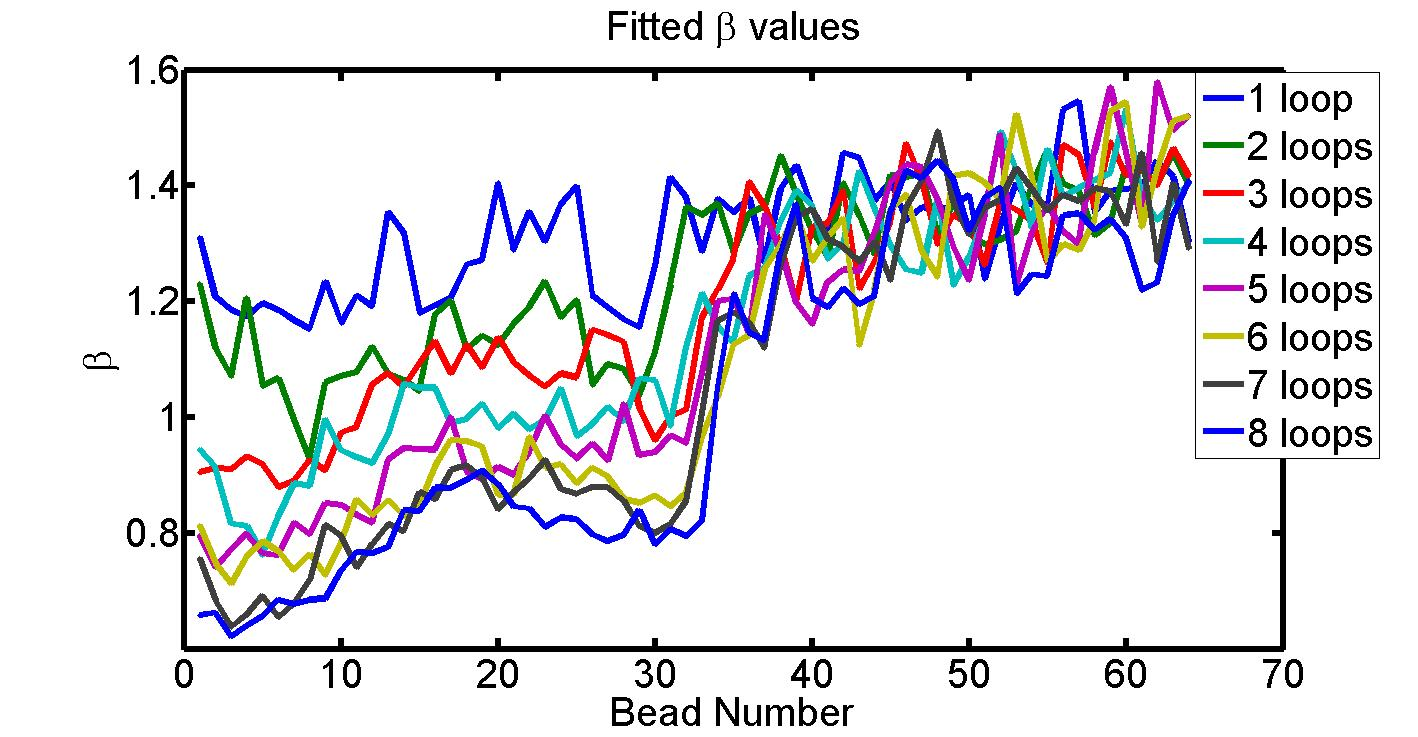
\includegraphics[scale=0.12]{fittedExpOneTAD1To8Loops}
\caption{\scriptsize{The encounter histogram (upper panel) of the case of random fixed loops in the region 1 to 32. As the number of random loops increases from 1 to 8 we see the emergance of a TAD region. The mean encounter probability (lower left panel) of the eight cases. The decrease in $\beta$ as the number of loops increases is attributed to the increased encounter between the first 32 beads. The fitted $\beta$ values (lower right panel) for the encounter data of each bead is displayed for the 8 cases.}}
\end{figure}

\subsection{Two TADS}
We follow similar procedure as with the one TAD simulation, only now we create random loops in two regions to form two TADs. The first regions is defined between bead 1 to 32, the second region between bead 33 to 64. In each simulation round we sequentially increase the number of random fixed loops from 1 to 10. 

\begin{figure}[H]
\centering
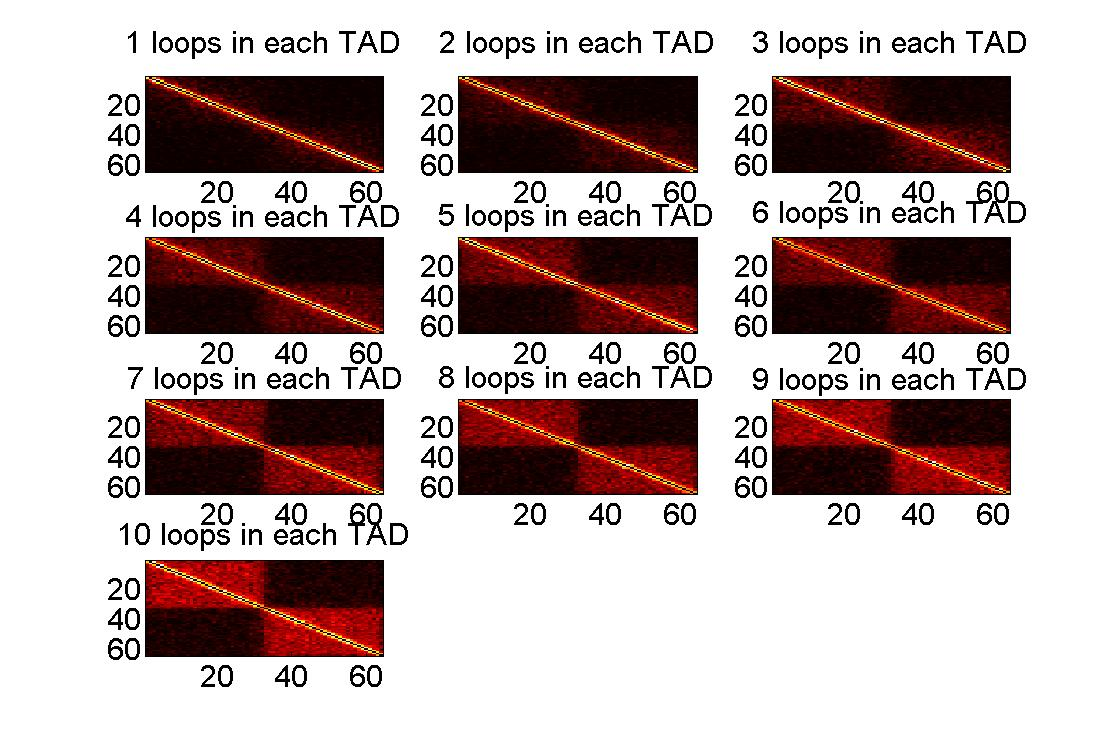
\includegraphics[scale=0.25]{encounterHistogram1To10LoopsInEachTAD}
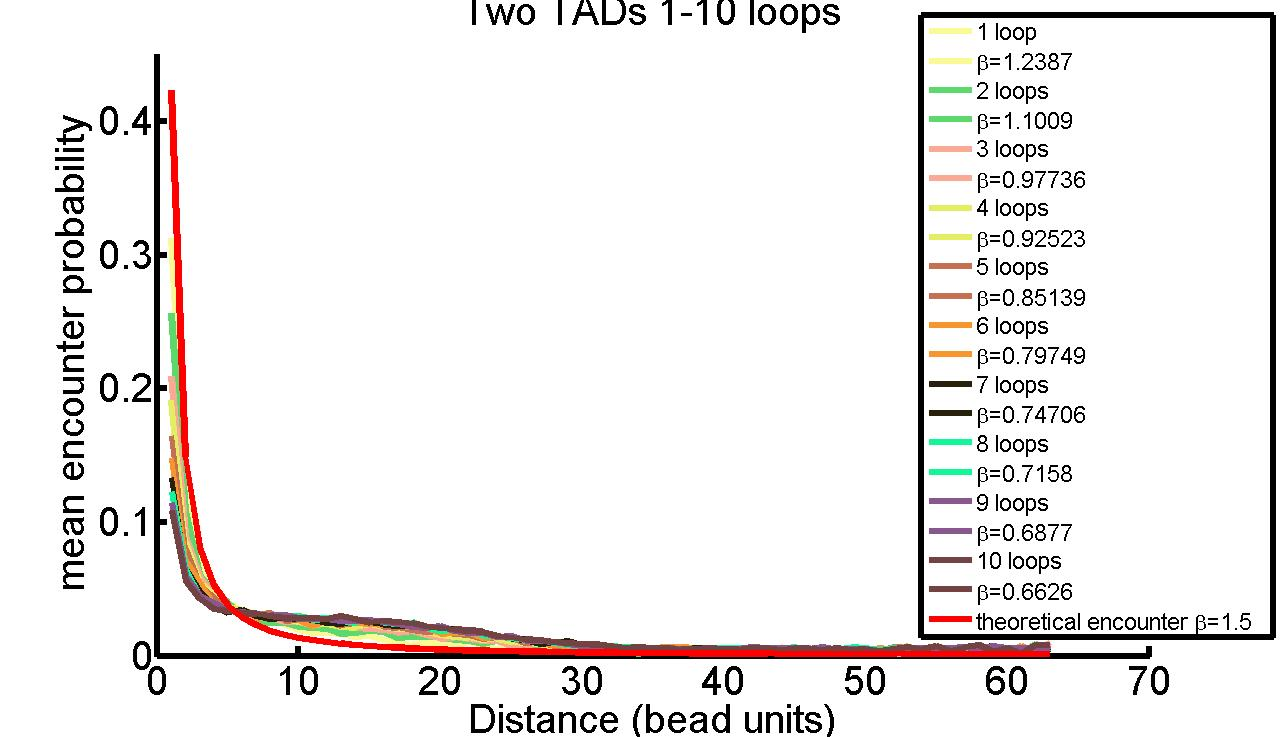
\includegraphics[scale=0.1]{meanEncounterProbabilityTwoTADs}
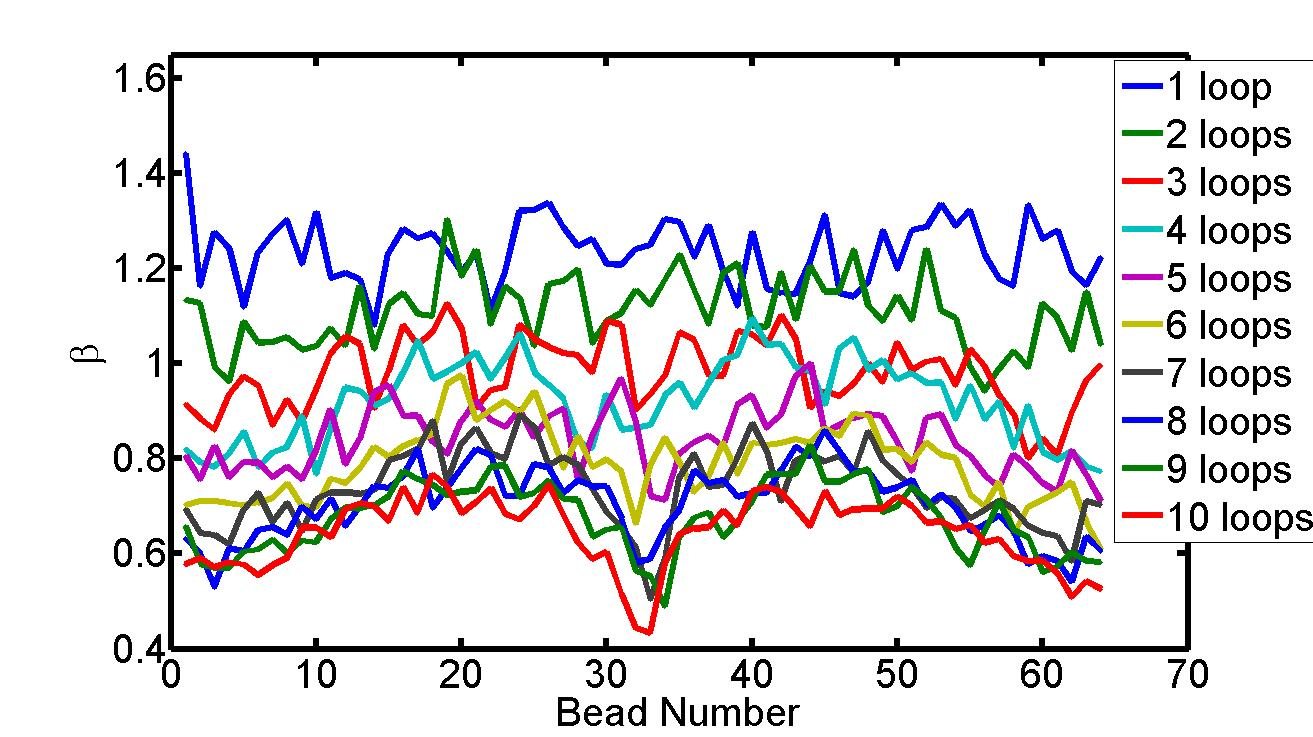
\includegraphics[scale=0.1]{fittedExpTwoTADs1To10Loops}
\caption{\scriptsize{The encounter histograms (upper panel) of the case with two TADs. As the number of loops in each TAD increases from 1 to 10, the two TADs emerges. The mean encounter probability (lower left panel) of the 10 cases resembles that of the one TAD case due to to 32 beads size of the TAD. The fitted $\beta$ values for the encounter probability of each bead in the 10 cases (lower right panel).}}
\end{figure}
 


\subsection{The conditional encounter probability of two beads and a loop}
We now turn to explore the conditional probability that a bead $B$ encounters bead $A$ before it encounter bead $C$ in a chain containing one loop. There are 27 configurations for the position of the beads in relation to the loop. Here we address the case of a chain with two equally sized tails. Thus, due to symmetry we reduce the possible configurations to 14. We term the beads contained in the loop as 'in the loop' and beads outside as beads 'on the tail'. The possible configurations are: 
\begin{enumerate}
\item $A$ in the loop, $B$ and $C$ on the same tail
\item $A$ in the loop, $B$ and $C$ on different tails
\item $B$ in the loop, $A$ and $C$ on the same tail
\item $B$ in the loop, $A$ and $C$ on different tails
\item $C$ in the loop, $A$ and $B$ on the same tail 
\item $C$ in the loop, $A$ and $B$ on different tails 
\item $A$ and $B$ in the loop, $C$ on the tail 
\item $A$ and $C$ in the loop, $B$ on the tail 
\item $B$ and $C$ in the loop, $A$ on the tail 
\item $A$, $B$ and $C$ in the loop
\item $A$, $B$ and $C$ are on the tail
\item $A$, $B$ on one tail, $C$ on the other tail
\item $A$, $C$ on one tail, $B$ on the other tail
\item $B$, $C$ on one tail, $A$ on the other tail
\end{enumerate}
The different cases are summarized graphically in Figure \ref{possibleArrangementOfThreeBeadsAndAloop}
\begin{figure}[H]
 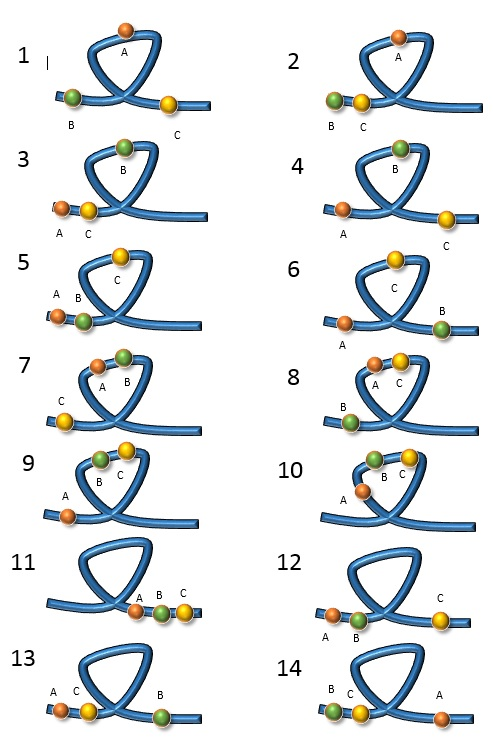
\includegraphics[scale=0.5]{possibleArrangementOfThreeBeadsAndAloop.jpg}
 \caption{\scriptsize{The possible configuration in the case of three beads and a loop, leaving tails of equal length}}\label{possibleArrangementOfThreeBeadsAndAloop}
\end{figure}
The conditional probability encounters and the mean first encounter time, are summarized in the Table \ref{conditionalEncouterProbabilityAndMFET}
according to the cases specified above
\begin{table}[H]

\begin{tabular}{l|l|l|l|l}
case & Bead A-B & MFET A-B (sec)&Bead B-C & MFET B-C (sec)\\
 \hline
1 & 0.15 & 0.34 & 0.85 & 0.23\\
2 & 0.76 & 3.97 & 0.23 & 3.11\\
3 & 0.37 & 1.47 & 0.63 & 1.46\\
4 & 0.53 & 1.79 & 0.47 & 2.25\\
5 & 0.86 & 0.29 & 0.16 & 0.15\\
6 & 0.29 & 2.57 & 0.71 & 4.14\\
7 & 0.79 & 0.55 & 0.21 & 0.45\\
8 & 0.63 & 1.83 & 0.37 & 2.20\\
9 & 0.26 & 0.46 & 0.74 & 0.81\\
10& 0.52 & 0.13 & 0.48 & 0.15\\
11& 0.54 & 0.14 & 0.46 & 0.11\\
12& 0.97 & 0.29 & 0.03 & 0.13\\
13& 0.56 & 8.39 & 0.44 & 6.19\\
14& 0.01 & 0.02 & 0.99 & 0.3
\end{tabular}
\caption{\scriptsize{Summary of the results of simulating the conditional probability that bead B meets A before C (Bead A-B), and probability that bead B meets C before A (Bead B-C), with the mean first encounter time (MFET) given in units of seconds. For each cse 10 simulation were performed}}\label{conditionalEncouterProbabilityAndMFET}
\end{table} 

\subsection{Conditional encounter of 3 beads in a linear chain}

In the analysis of the experimental data as performed by Giorgetti et al, 3 loci were found to be significant to the internal organization of TAD D. These loci overlap the position of the highly interacting Xite/Tsix, Chic1, and Linx. , which correspond to beads in the range 25-27, 33-35, and 86-89 respectively.

We therefore simulate a 108 beads chain and assess the conditional probability that  bead 34 (Chic1) encounter bead 26 (Xite/Tsix) before bead 87 (Linx). All simulations were ran until an encounter occurred. time step was set to $8.3\times 10^{-5}$ [sec]. The encounter distance was set to $b/5=0.02$, where $b$ is the standard-deviation of the distance between adjacent beads. 

\subsection{Conditional encounter of 3 beads in the random loop model}


\end{document}